\chapter{Revisão Bibliográfica}

No presente capítulo, são apresentados conceitos básico para a compreensão do trabalho. Nessa etapa, busca-se através da revisão de trabalhos já elucidados a contextualização do projeto proposto.

%%%%%%%%%%%%%%%%%%%%%%%%%%%%%%%%%%%%%%%%%%%%%%%%%%%%%%%%%%%%%%%%%%%%%%

\section{Satélites Artificiais} %ch 1303

Desde o lançamento do satélite Sputnik I, primeiro satélite artificial, que foi desenvolvido e lançado pela extinta URSS (União das Repúblicas Socialistas Soviéticas) no dia 4 de Outubro de 1957, novas formas de controle foram desenvolvidas. Como o principal fim de um satélite é a comunicação e a navegação, que exigem orientação acurada, juntamente com todas as forças que atuam sobre o satélite, se torna imprescindível o uso de técnicas de controle para se garantir a translação e a rotação do satélite \cite{Brown2002}. Na figura \ref{fig:rotational_brown_p256}, podemos ver os movimentos de rotação e translação de um satélite ao redor de um planeta.

\begin{figure}[!ht]
  \caption{Movimento de Translação de um satélite Artificial.}
  \begin{center}
      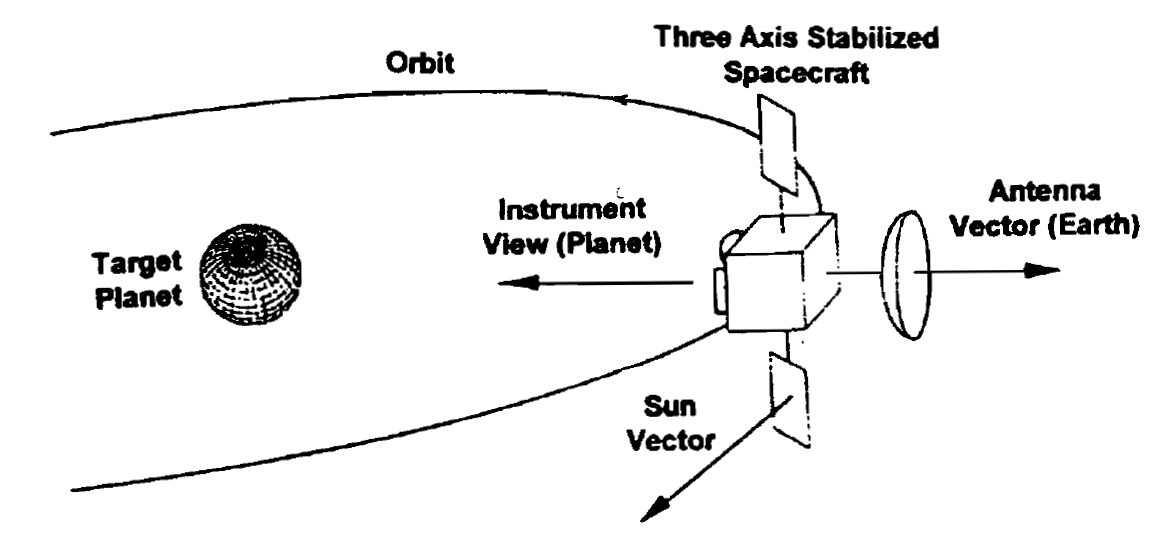
\includegraphics[scale=0.5]{img/rotational_brown_p256}
  \end{center}
  \fonte{Adaptado de \citeonline{Brown2002}.} 
  \label{fig:rotational_brown_p256}
\end{figure}

%%%%%%%%%%%%%%%%%%%%%%%%%%%%%%%%%%%

\subsection{Dinâmica de um Satélite}

A dinâmica é dividida em duas partes, onde uma representa os movimentos de translação e a outra os de rotação.


%%%%%%%%%%%%%%%%%%%%%%%%%%%%%%%%%%%

\subsubsection{Dinâmica de Translação}

A dinâmica de translação de um copo em relação ao outro é um caso de \textit{Dinâmica de Corpo Rígido}. A fundação da Dinâmica de corpos rígidos foi feita pelo Físico Inglês Isaac Newton em forma de três leis, das quais, a 2º e a 3ª são primordiais para descrever a dinâmica de rotação \cite{Snider}. A 2ª lei de Newton pode ser escrita das seguintes forma:

\begin{equation}\label{eq:fma}
  \vec{F}=\frac{d}{dt}\vec{p}\quad\quad\quad\quad\vec{p}=m\vec{v}
\end{equation}

\begin{equation}
  \vec{F}=m\vec{a}
\end{equation}

Onde $\vec{F}$ é a força, $\vec{p}$ é o momento linear, $\vec{v}$ é a velocidade e $\vec{a}$ é  aceleração. Ainda, podemos descrever a força total sobre uma partícula $\vec{F_i}$ da seguinte forma:

\begin{equation}\label{eq:Fi}
\vec{F_i}=\vec{f_{ie}}+\sum_{i\neq j}^{N}{\vec{f_{ie}}} = m_i\vec{a_i}
\end{equation}
 
 Onde, $\vec{f_{ie}}$ é a força externa e $\vec{f_{ij}}$ é a força interna de carda parte j que compõe o corpo i e $m_i\vec{a_i}$ é a massa e a força resultante no corpo rígido.

 Ao unirmos N partículas para formar um corpo rígido, estamos somando todas as forças externas e as forças internas de todos os corpos da seguinte forma:

\begin{equation}
  \sum_{i=1}^{N}{\vec{F_i}}=\sum_{i=1}^{N}{\vec{f_i}}+\sum_{i=1}^{N}{\sum_{i\neq j}^{N}{\vec{f_i}j=}}\sum_{i=1}^{N}{m_i\vec{a_i}} 
\end{equation}

Segundo a 3ª Lei de Newton, como o corpo j exerce uma força $\vec{f_{ji}}$ em módulo igual a força $\vec{f_{ij}}$ que o corpo i exerce sobre o corpo j, só que oposta. Logo, as forças internas se anulam.  

Quando temos um conjunto de partículas unidas, podemos descrever a força total sobre o corpo ($\vec{F_e}$) como o somatório de todas as forças sobre as partículas ($\vec{F_{ie}}$). Isso pode ser esquito da seguinte forma:

\begin{equation}\label{eq:fet}
  \vec{F_{e}}=\sum_{i=1}^{N}{\vec{f_{ie}}}=\sum_{i=1}^{N}{m_i\vec{a_i}} 
\end{equation}

A imagem \ref{fig:translacao_referencial_snider_p15}, representa o vetor posição $\vec{r_{com}}$ de um corpo rígido em relação a origem. A descrição matemática desse vetor pode ser visto na equação \ref{eq:rcom}.

\begin{figure}[!ht]
  \caption{Representação de $\vec{r_{com}}$}
  \begin{center}
      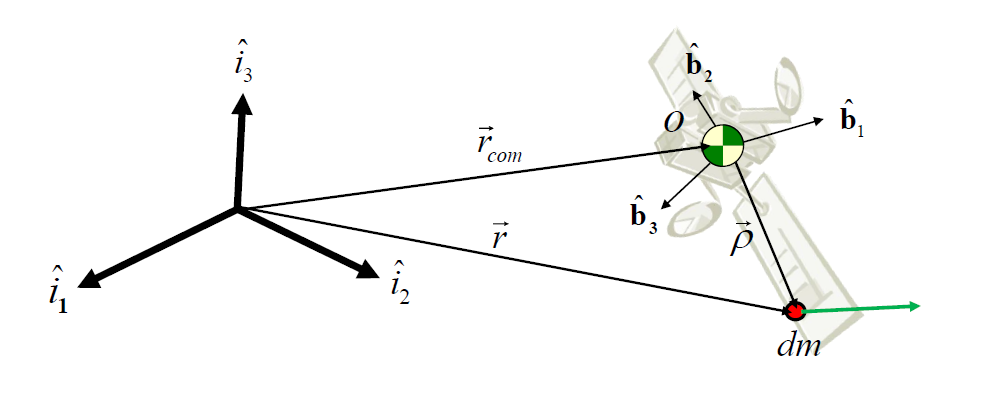
\includegraphics[scale=0.5]{img/translacao_referencial_snider_p15}
  \end{center}
  \fonte{Adaptado de \citeonline{Snider}.} 
  \label{fig:translacao_referencial_snider_p15}
\end{figure}

\begin{equation}\label{eq:rcom}
  \vec{r_{com}}=\frac{1}{M_T}\sum_{i=1}^{N}{m_i\vec{r_i}} 
\end{equation}

Onde, $M_T$ é a massa total do corpo rígido.

Como a aceleração é a derivada segunda da posição, derivamos duas vezes a posição $\vec{r_{com}}$ e multiplicamos pela massa total em ambos os lado da equação \ref{eq:rcom}. Assim temos:

\begin{equation}\label{eq:2deriv}
  M_T\frac{{d}^{2}}{{d}t^{2}}\vec{r_{com}}=\sum_{i=1}^{N}{m_i\vec{a_i}}
\end{equation}

Igualando as equações \ref{eq:fet} e \ref{eq:2deriv}, temos a força total sobre um corpo rígido que desempenha movimento de translação. Isso pode ser visto na sequência.

\begin{equation}
\vec{F_e}=M_{T}\frac{{d}^{2}}{{d}t^{2}}\vec{r_{com}} 
\end{equation}


%%%%%%%%%%%%%%%%%%%%%%%%%%%%%%%%%%%

\subsubsection{Dinâmica de Rotação}

A dinâmica de rotação descreve o movimento de um corpo rígido em relação a um ponto. Para descrevermos os movimentos de rotação, devemos conhecer a distribuição de massa do corpo rígido \cite{Snider}. A figura \ref{fig:mass_snider_p16} ilustra a distribuição de massa infinitesimal de um corpo tridimensional. 

\begin{figure}[!ht]
  \caption{Distribuição de Massa}
  \begin{center}
      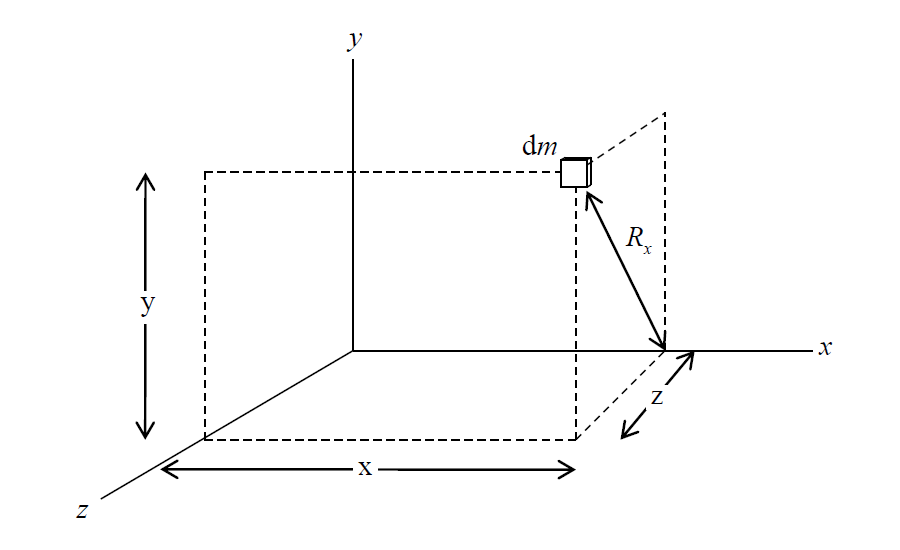
\includegraphics[scale=0.5]{img/mass_snider_p16}
  \end{center}
  \fonte{Adaptado de \citeonline{Snider}.} 
  \label{fig:mass_snider_p16}
\end{figure}

Por definição, o momento de inércia infinitesimal disposto sobre um eixo ($I_{xx}$, $I_{yy}$ e $I_{zz}$) é o produto da massa pela distância do ponto de referência. Se fizermos isso mara N partículas, temos:

\begin{equation}
  I_{xx}=\sum_{i=1}^{N}{m_i({y_i}^{2}+{z_i}^{2})}
\end{equation}

\begin{equation}
  I_{yy}=\sum_{i=1}^{N}{m_i({x_i}^{2}+{z_i}^{2})}
\end{equation}

\begin{equation}
  I_{zz}=\sum_{i=1}^{N}{m_i({x_i}^{2}+{y_i}^{2})}
\end{equation}

Já quando as partículas estão dispostas sobre os planos xy, xz e yz, temos:

\begin{equation}
  I_{xy}=-\sum_{i=1}^{N}{m_ix_iy_i}=I_{xy}
\end{equation}

\begin{equation}
  I_{xz}=-\sum_{i=1}^{N}{m_ix_iz_i}=I_{zx}
\end{equation}

\begin{equation}
  I_{yz}=-\sum_{i=1}^{N}{m_iy_iz_i}=I_{zy}
\end{equation}

Com isso, podemos criar uma matriz que representa o momento de inércia total do corpo rígido:

\begin{equation}\label{eq:nsimetrico}
I=\begin{bmatrix}I_{xx}&I_{xy}&I_{xz}\\I_{yx}&I_{yy}&I_{yz}\\I_{zx}&I_{zy}&I_{zz}\end{bmatrix}
\end{equation}

Caso o satélite seja simétrico, os momentos de inércia nos planos xy, xz e yz são de mesmo módulo só que com sinal oposto aos momentos de inércia dos planos xy, zx e zy, anulando todos esses termos. Isso pode ser visto na seguinte matriz diagonal:

\begin{equation}
I=\begin{bmatrix} I_{ xx } & 0 & 0 \\ 0 & I_{ yy } & 0 \\ 0 & 0 & I_{ zz } \end{bmatrix}=\begin{bmatrix} A & 0 & 0 \\ 0 & B & 0 \\ 0 & 0 & C \end{bmatrix}
\end{equation}

Para facilitar a escrita das equações, os momentos de inércia $I_{xx}$, $I_{yy}$ e $I_{zz}$ serão descritos como A, B e C respectivamente.

Após a descrição matemática do momento de inércia, podemos começar a analisar o movimento de rotação do corpo rígido. Vamos começar pela velocidade angular instantânea $\omega$, que pode ser descrita como a derivada primeira da posição $\beta$ angular, segundo o teorema fundamental do cálculo:

\begin{equation}
\omega\equiv\lim_{\Delta t\rightarrow 0}\frac{\Delta\beta}{\Delta t}=\frac{d\beta}{dt}
\end{equation}

A aceleração angular $\alpha$, nada mais é do que a primeira derivada da velocidade angular:

\begin{equation}
\alpha\equiv\lim_{\Delta t\rightarrow 0}\frac{\Delta\omega}{\Delta t}=\frac{d\omega}{dt}
\end{equation}

Outra equação importante para descrever a maioria dos tipos de movimento, é aquela que relaciona a posição $\beta$ com a posição inicial $\beta_0$, velocidade angular inicial $\omega_0$, o tempo inicial do movimento $t_0$, o tempo atual t e a aceleração angular $\alpha$. A expressão pode ser vista na sequência.

\begin{equation}
\beta=\beta_{0}+\omega_{0}(t-t_{0})+\frac{1}{2}\alpha{(t-t_{0})}^{2}
\end{equation}

Não menos importante, é a expressão que relaciona a velocidade angular $\omega$ com a velocidade angular inicial $\omega_0$, aceleração angular e o deslocamento ($\beta-\beta_0$). Isso é descrito na equação da sequência.

\begin{equation}
{\omega}^{2}={\omega_0}^{2}+2\alpha(\beta-\beta_0) 
\end{equation}

Como foi feito na dinâmica de translação, precisamos relacionar os momentos e a aceleração angular $\alpha$. Para isso vamos começar relacionando o torque $\vec{\tau}$ com a derivada do momento angular $\vec{L}$:

\begin{equation}
\vec{\tau}=\dot{\vec{L}}
\end{equation}

Mas como o momento angular é o produto do momento de inércia do corpo I pela velocidade angular, assim: 

\begin{equation}\label{eq:iomega}
\vec{L}=I\vec{\omega}
\end{equation}

Com isso, já conhecendo as relações entre velocidade e aceleração, temos:  

\begin{equation}\label{iomega}
\vec{\tau}=I\dot{\vec{\omega}}=I\vec{\alpha}
\end{equation}

Se usarmos o teorema do transporte cinemático, o momento de inércia pode ser escrito da seguinte forma:

\begin{equation}
\dot{\vec{L}}=I\dot{\vec{\omega}}+\vec{\omega}\times I \vec{\omega}
\end{equation}

Por consequência, descrevemos o torque da seguinte maneire:

\begin{equation}\label{eq:torque}
\vec{\tau}=I\dot{\vec{\omega}}+\vec{\omega}\times I \vec{\omega}
\end{equation}

Como temos o momento de inércia do corpo rígido representado em forma de matriz, precisamos mudar a representação a matricial. Começaremos pela velocidade angular $\vec{\omega}$, que em módulo, pode ser descrita da seguinte forma:

\begin{equation}
\left|\vec{\omega}\right|=\begin{bmatrix}\omega_1\\\omega_2\\\omega_2\end{bmatrix}
\end{equation}

Se fizermos o mesmo com a equação \ref{eq:torque}, temos:

\begin{equation}
\begin{bmatrix}\tau_{1}\\\tau_{2}\\\tau_{3}\end{bmatrix}=\begin{bmatrix}A\dot{\omega}_{1}\\B\dot{\omega}_{2}\\C\dot{\omega}_{3}\end{bmatrix}+\begin{bmatrix}\omega_{1}\\\omega_{2}\\\omega_{3}\end{bmatrix}\times\begin{bmatrix}A\omega_{1}\\B\omega_{2}\\C\omega_{3}\end{bmatrix}
\end{equation}

Como podemos ver, já conseguimos relacionar os momentos de inércia do corpo rígido simétrico com as demais variáveis de interesse. Ainda, podemos sair da forma matricial e apresentarmos os torques da forma algébrica, isso pode ser visto nas 3 equações a seguir.

\begin{equation}
  \tau_1=A\dot{\omega_1}-(B-C)\omega_2\omega_3 
\end{equation}

\begin{equation}
  \tau_2=B\dot{\omega_2}-(C-A)\omega_1\omega_3 
\end{equation}

\begin{equation}
  \tau_3=C\dot{\omega_3}-(A-B)\omega_1\omega_2
\end{equation}

Se utilizarmos um corpo não simétrico, podemos recorrer a matriz da equação \ref{eq:nsimetrico}, e obteremos as 3 seguintes equações para descrever o torque:

\begin{equation}\label{eq:torquexyz}
 \tau_{1}=I_{xx}\dot{\omega_{1}}-I_{xy}(\dot{\omega_{2}}-\omega_{1}\omega_{3})-I_{xz}(\dot{\omega_{3}}+\omega_{1}\omega_{2})\\-(I_{yy}-I_{zz})\omega_{2}\omega_{3}-I_{yz}({\omega_{2}}^{2}-{\omega_{3}}^{2})
\end{equation}

\begin{equation}\label{eq:torquexyz2}
  \tau_{2}=I_{zz}\dot{\omega_{3}}-I_{yz}(\dot{\omega_{3}}-\omega_{1}\omega_{2})-I_{xy}(\dot{\omega_{1}}+\omega_{2}\omega_{3})\\-(I_{zz}-I_{xx})\omega_{1}\omega_{3}-I_{xz}({\omega_{3}}^{2}-{\omega_{1}}^{2})
\end{equation}

\begin{equation}\label{eq:torquexyz3}
 \tau_{3}=I_{zz}\dot{\omega_{1}}-I_{xz}(\dot{\omega_{1}}-\omega_{2}\omega_{3})-I_{yz}(\dot{\omega_{2}}+\omega_{1}\omega_{3})\\-(I_{xx}-I_{yy})\omega_{1}\omega_{2}-I_{xy}({\omega_{1}}^{2}-{\omega_{2}}^{2})
\end{equation}

Se isolarmos a derivada da velocidade angular na nas equações \ref{eq:torquexyz}, \ref{eq:torquexyz2} e \ref{eq:torquexyz3}, conseguimos a relação da velocidade com o torque aplicado. Isso pode ser visto nas 3 seguintes equações:

\begin{equation}
  \dot{\omega_{1}}=\frac{\tau_{1}}{A}+\left(\frac{B-C}{A}\right)\omega_{2}\omega_{3}
\end{equation}

\begin{equation}
  \dot{\omega_{2}}=\frac{\tau_{2}}{B}+\left(\frac{C-A}{B}\right)\omega_{1}\omega_{3}
\end{equation},

\begin{equation}
  \dot{\omega_{3}}=\frac{\tau_{2}}{C}+\left(\frac{A-B}{C}\right)\omega_{1}\omega_{2}
\end{equation}


%%%%%%%%%%%%%%%%%%%%%%%%%%%%%%%%%%%%%%%%%%%%%%%%%%%%%%%%%%

\subsubsection{Matrizes de Rotação e Ângulos de Euler}

Na seção anterior, temos como resultado 3 equações diferenciais ordinárias de primeira ordem (EDO), também chamadas de equações de Euler. Essas equações definem a dinâmica do corpo rígido em relação a um ponto fixo. Como temos o interesse de controle de posição, ainda nos falta uma relação matemática para expressar a posição angular $\beta$, velocidade angular $\omega$ e a aceleração $\alpha$, isso em um espaço tridimensional \cite{Snider}.

Na imagem \ref{fig:coordenada}, podemos ver a representação dos ângulos de Euler ($\psi, \theta, \phi$) em relação aos eixos $b_1, b_2 e b_3$, oriundos de uma transformação pela sequência de Euler \cite{BongWie2001}.

\begin{figure}[!ht]
  \caption{Ângulos de Euler}
  \begin{center}
      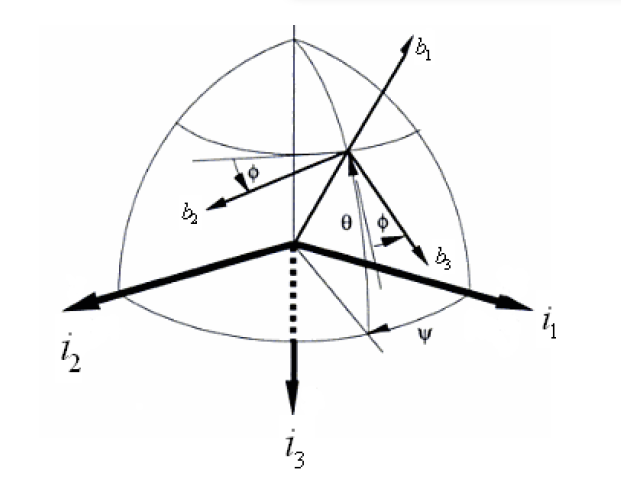
\includegraphics[scale=0.5]{img/euler_snider_p28}
  \end{center}
  \fonte{Adaptado de \citeonline{Snider}.} 
  \label{fig:coordenada}
\end{figure}

As duas matrizes de rotação obtidas pelo trabalho de Euler podem ser vistas na sequência: 

\begin{equation}
\begin{bmatrix} \dot { \phi  }  \\ \dot { \theta  }  \\ \dot { \psi  }  \end{bmatrix}=\frac { 1 }{ cos\theta  } \begin{bmatrix} cos\theta  & sen\phi sen\theta  & cos\phi sen\theta  \\ 0 & cos\phi cos\theta  & -sen\phi cos\theta  \\ 0 & sen\phi  & cos\phi  \end{bmatrix}\begin{bmatrix} \omega_1 \\ \omega_2  \\ \omega_3  \end{bmatrix} 
\end{equation}

\begin{equation}
\begin{bmatrix} \dot { \phi  }  \\ \dot { \theta  }  \\ \dot { \psi  }  \end{bmatrix}=\frac { 1 }{ sin\theta  } \begin{bmatrix} sen\psi  & cos\psi  & 0 \\ cos\psi sen\theta  & -sen\psi sen\theta  & 0 \\ -sen\psi cos\theta  & -cos\psi cos\theta  & 0 \end{bmatrix}\begin{bmatrix} \omega _{ 1 } \\ \omega _{ 2 } \\ \omega _{ 3 } \end{bmatrix}
\end{equation}


%%%%%%%%%%%%%%%%%%%%%%%%%%%%%%%%%%%%%%%%%%%%%%%%%%%%%%%%%%%%%%

\subsubsection{Rodas de Reação}

Uma rodas de reação consiste em um rotor que é fixado em satélites ou em outros veículos, com o objetivo de mudar a posição dos mesmos através da variação de velocidade da roda, criando uma reação pela criação de um torque. Quando a roda sofre uma desaceleração, ela exerce um torque em uma direção, se acelerada, em outra \cite{BongWie2001}. Na figura \ref{fig:satellite_controlhand_p1306} podemos ver 3 rodas de reação dispostas nos 3 eixos de um corpo rígido.

\begin{figure}[!ht]
  \caption{Representação Mecânica Simplificada de um satélite com rodas de Reação.}
  \begin{center}
      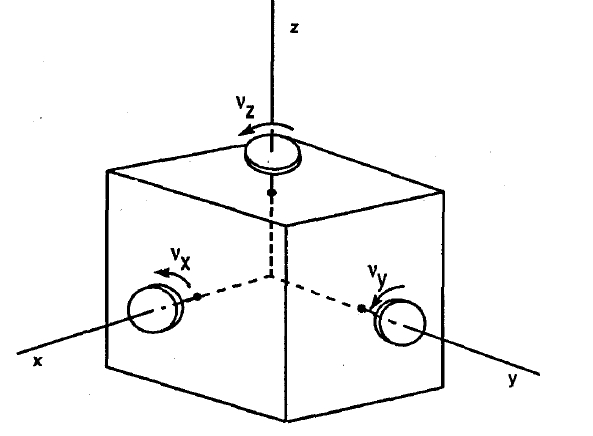
\includegraphics[scale=0.75]{img/satellite_controlhand_p1306}
  \end{center}
  \fonte{Adaptado de \citeonline{Levine1996}.} 
  \label{fig:satellite_controlhand_p1306}
\end{figure}

Como já foram descritos nas outras seções, precisamos encontrar uma relação que expresse o torque criado pelas rodas de reação, para que consigamos unir ao modelo do satélite. Para isso começamos pelo momento angular total $\vec{L_{tot}}$, que pode ser visto na sequência.

\begin{equation}\label{eq:ltot}
\vec{L_{tot}}=\vec{L_s}+\vec{L_{\omega}}=constante 
\end{equation}

Onde $L_s$ representa o momento angular do satélite e $\vec{L_{\omega}}$ o momento angular da roda de reação. Como já vimos na equação \ref{eq:iomega}, o momento angular pode ser descrito da seguinte forma:

\begin{equation}
\vec{L_s}=I\vec{\omega}
\end{equation}

E o momento angular nas rodas de ração podem ser escritos da seguinte forma:

\begin{equation}
\vec {L_{\omega} } =D_{\omega}\vec{\psi_{\omega}} 
\end{equation}

Onde $D_{\omega}$ é o momento de inércia da roda de reação e $\vec{\psi_{\omega}}$ é variação instantânea da posição angular da roda. Com isso, conseguimos encontrar o torque promovido pela roda de reação $\tau_{\omega}$:

\begin{equation}\
\vec{\tau_{\omega}}=\dot{\vec{L_{\omega}}}=D_{\omega}\dot{\vec{\psi_{\omega}}}
\end{equation}

E por fim, podemos relacionar o torque da roda com o do satélite e todas as outras variáveis de interesse. Para isso é usada a equação \ref{eq:ltot} e a relação entre torque e momento angular da equação anterior. O resultado pode ser visto nas 3 equações seguintes:

\begin{equation}\label{eq:torquefinal1}
\tau_{1}=A\dot{\omega_{1}}+(D_{\omega}\dot{\psi_{\omega}})_{1}+(C-B)\omega_{2}\omega_{3}-(D_{\omega}\psi_{\omega})_{2}\omega_{3}+(D_{\omega}\psi_{\omega})_{3}\omega_{2}
\end{equation}

\begin{equation}\label{eq:torquefinal2}
\tau_{2}=B\dot{\omega_{2}}+(D_{\omega}\dot{\psi_{\omega}})_{2}+(A-C)\omega_{1}\omega_{3}+(D_{\omega}\psi_{\omega})_{2}\omega_{3}-(D_{\omega}\psi_{\omega})_{3}\omega_{1}
\end{equation}

\begin{equation}\label{eq:torquefinal3}
\tau_{3}=C\dot{\omega_{3}}+(D_{\omega}\dot{\psi_{\omega}})_{3}+(B-A)\omega_{1}\omega_{2}-(D_{\omega}\psi_{\omega})_{1}\omega_{2}+(D_{\omega}\psi_{\omega})_{3}\omega_{1}
\end{equation}

%%%%%%%%%%%%%%%%%%%%%%%%%%%%%%%%%%%%%%%%%%%%%%%%%%%%%%%%%%%%%%%%%%%%%%

\section{Controlador PID}

\subsection{Resposta ao Degrau do um Sistema}

Um problema fundamental em engenharia, é prever e modelar sistemas naturais ou artificias para tirarmos o melhor proveito de suas características. Para isso, muitas técnicas foram desenvolvidas para se conseguir controlar essas variáveis de interesse \cite{Levine1996}.

Uma forma clássica de representar um resposta de uma variável de interesse, é através da resposta ao degrau. Essa pode ser vista na figura \ref{fig:transient_ogata_p170}, onde temos as principais características da resposta ao degrau de um sistema de segunda ordem ou superior. Onde \textit{$M_p$} (maximum overshoot) é o sobressinal do da variável de interesse em percentual, \textit{$t_d$} (delay Time) é o tempo atraso de transporte, \textit{$t_r$} (rise time) é o tempo necessário para atingir o valor do sinal de referência, \textit{$t_p$} é o tempo de pico (peak time) e \textit{$t_s$} (settling time) é o tempo para o sistema entrar em regime, observando um critério de erro em regime \cite{Ogata}.

\begin{figure}[!ht]
  \caption{Parâmetros de uma Resposta ao Degrau de um sistema de segunda ordem ou superior.}
  \begin{center}
      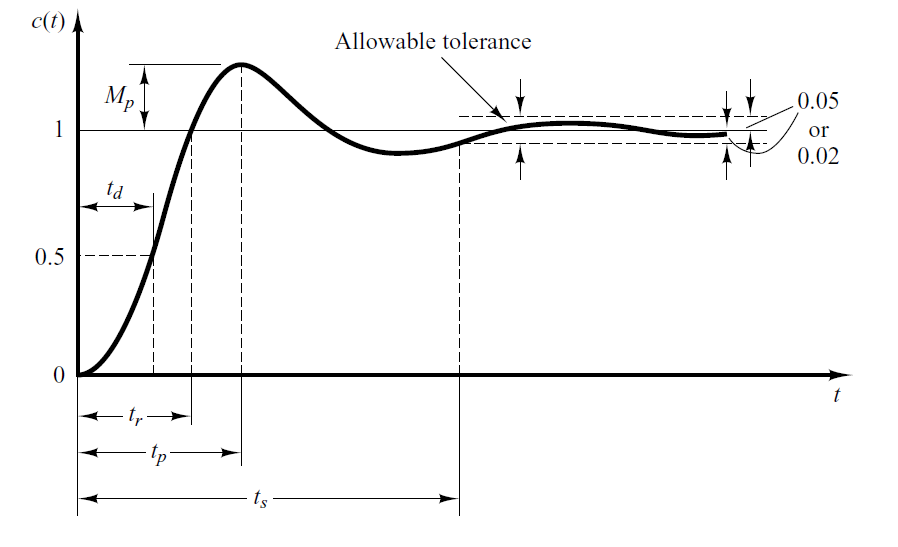
\includegraphics[scale=0.5]{img/transient_ogata_p170}
  \end{center}
  \fonte{Adaptado de \citeonline{Ogata}.} 
  \label{fig:transient_ogata_p170}
\end{figure}

A resposta ao degrau nos diz muito sobre os sistemas de interesse, pois nela podemos ver claramente a atuação dos \textit{polos} e \textit{zeros} dominantes e o ganho de baixa frequência da função de transferência do sistema. Os métodos clássicos para se calcular os parâmetros de controladores são baseados na resposta ao degrau \cite{Ogata}. 


%%%%%%%%%%%%%%%%%%%%%%%%%%%%%%%%%%%

\subsection{Controlador PID}

O controlador proporcional-integral-derivativo é um dos controladores mais utilizados nas aplicações industriais. Essa topologia de controlador consegue, em diferentes configurações atender entre 90 e 95\% de todos os sistemas que necessitam de controladores \cite{Levine1996}. A forma descritiva matemática mais comum de se encontrar um controlador PID no domínio do tempo é a seguinte:

\begin{equation}
  u(t) = K\left((e(t)+\frac{1}{T_i}\int_{0}^{t}{e(\tau)}d\tau+T_d\frac{de(t)}{dt}\right) 
\end{equation}

Onde \textit{e(t)} é o erro, \textit{$T_i$} é o tempo integral, \textit{$T_d$} é o tempo derivativo e \textit{K} o ganho proporcional. Uma outra forma de se representar os tempos integral e derivativo, é através dos ganhos \textit{$K_i$} que é o ganho integral e o \textit{$K_d$}, que é o ganho derivativo \cite{Astrom1995};

A partir desse princípio podemos relacionar com as equações \ref{eq:torquefinal1}, \ref{eq:torquefinal2} e \ref{eq:torquefinal3} podemos escrever a relação do controlador PID do Torque do motor:

\begin{equation}
\tau_{m_{1,2,3}}=K_{P}\left((\beta_{com}-\beta)+\frac{1}{T_{I}}\int{(\beta_{com}-\beta)dt}+T_{d}\frac{d}{dt}(\beta_{com}-\beta)\right)
\end{equation}

\begin{equation}
=K_{P}\left(\beta_{com}+\frac{1}{T_{I}}\int{\beta_{com}dt}+T_{d}\frac{d}{dt}\beta_{com}\right) 
\end{equation}

Na figura \ref{fig:pid_controller_Snider_p35}, podemos ver a configuração mais utilizada do controlador PID, onde $\beta_{com}(S)$ é o valor do sinal de referência no domínio da frequência, \textit{err(S)} o erro, \textit{$K_p$} é o ganho proporcional, \textit{$K_i$} é o ganho integral, \textit{$K_d$} é o ganho derivativo, \textit{$G_e(s)$} é a função de transferência do controlador PID, \textit{$M_{c1}(s)$} é o sinal de erro tratado pelo controlador, \textit{D(S)} é um distúrbio, \textit{$G_p(S)$} é a função de transferência da planta e por fim, \textit{$\beta(S)$} que é a variável de interesse \cite{Snider}.

\begin{figure}[!ht]
  \caption{Representação do Modelo de Controlador PID com distúrbios.}
  \begin{center}
      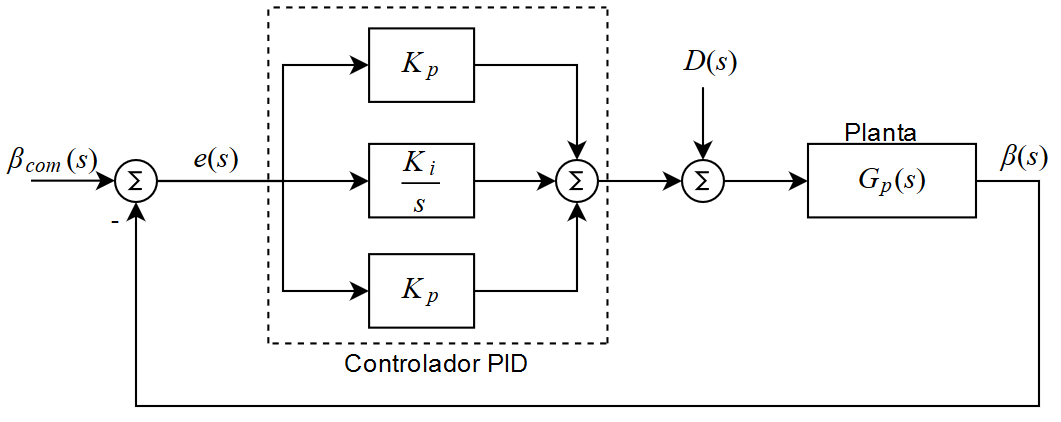
\includegraphics[scale=0.75]{img/pid_controller_Snider_p35}
  \end{center}
  \fonte{\citeonline{Snider}.} 
  \label{fig:pid_controller_Snider_p35}
\end{figure}

Como alguns sistemas podem admitir grandes e rápidas variações de sinais de referência, exigindo uma grande força de controle e energia no atuador, algumas topologias foram desenvolvidas para limitar a atuação de alguns fatores dos controladores. Um bom exemplo é o \textit{anti-windup}, onde essa topologia limita a saturação do atuador quando o sistema atinge o regime, causado pela ação integral. Essa topologia pode ser vista no modelo da figura \ref{fig:pid_antiwindup_astrom_p83} \cite{Astrom1995}.

\begin{figure}[!ht]
  \caption{Modelo de um Controlador PID com Histerese}
  \begin{center}
      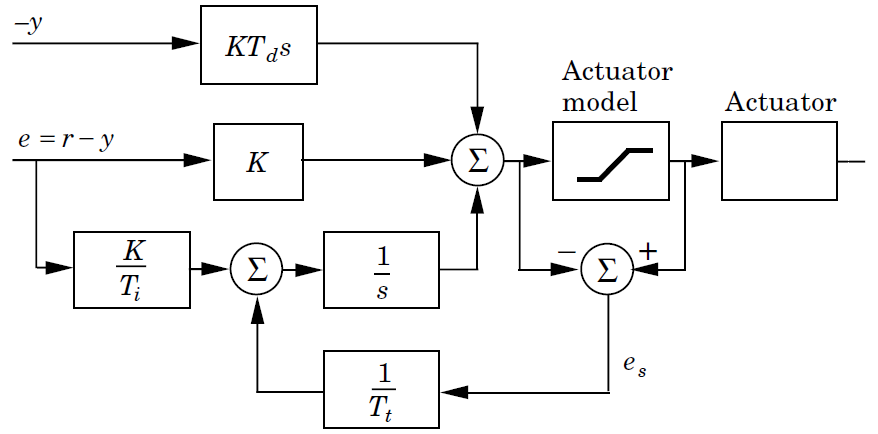
\includegraphics[scale=0.65]{img/pid_antiwindup_astrom_p83}
  \end{center}
  \fonte{\citeonline{Astrom1995}.} 
  \label{fig:pid_antiwindup_astrom_p83}
\end{figure}

Existem muitas combinações de controladores PID, cada uma com suas peculiaridades e vantagens de uso. Uma combinação muito usada é a PI, onde a acão integral de zerar o erro em regime e uma boa resposta transitória já satisfazem as especificações. Podemos ver um exemplo dessa configuração na imagem \ref{fig:pi_twomotors_astrom_p308}, onde apenas um controlador PI controla a velocidade angular (\textit{$\omega$})somada de dois motores (Motor 1 e Motor 2) a partir de uma velocidade de referência (\textit{$\omega_{sp}$}) \cite{Astrom1995}.

\begin{figure}[!ht]
  \caption{Representação do Modelo de Controlador PI com dois motores.}
  \begin{center}
      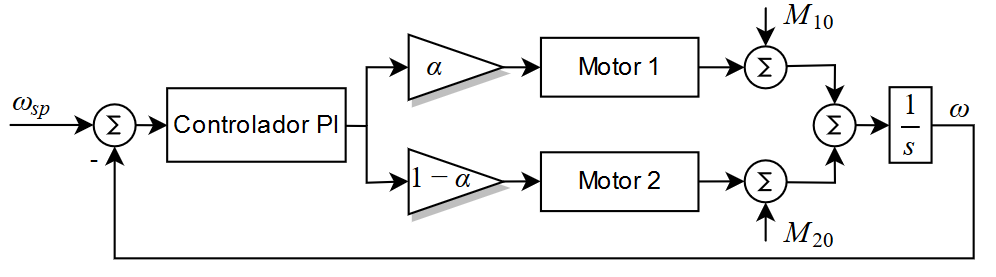
\includegraphics[scale=0.65]{img/pi_twomotors_astrom_p308}
  \end{center}
  \fonte{Adaptado de \citeonline{Astrom1995}.} 
  \label{fig:pi_twomotors_astrom_p308}
\end{figure}


%%%%%%%%%%%%%%%%%%%%%%%%%%%%%%%%%%%%%%%%%%%%%%%%%%%%%%%%%%%%%%%%%%%%%%

\section{Sintonia de Controladores}

Como podemos ver no modelo matemático e gráfico dos controladores PID, os valores de ajuste $K_p$, $T_i$ e $T_d$  podem assumir infinitos valores, sendo necessário a escolha do melhor conjunto desses valores para que a planta desempenhe o comportamento esperado \cite{Ogata}.


%%%%%%%%%%%%%%%%%%%%%%%%%%%%%%%%%%%

\subsection{Método de sintonia de Ziegler-Nichols}

Dois métodos clássicos de sintonia foram desenvolvidos em 1942 por Ziegler e Nichols. Esses dois métodos são baseados em características da resposta ao degrau e o com a resposta em frequência. Na figura \ref{fig:ziegler-nichols_astrom_p135} podemos ver a resposta ao degrau e os parâmetros de atraso (L) e velocidade da resposta (a), que são usados para o cálculos dos parâmetros do controlador  \cite{Astrom1995}. 

\begin{figure}[!ht]
  \caption{Resposta ao degrau e os parâmetros de atraso (L) e velocidade da resposta (a).}
  \begin{center}
      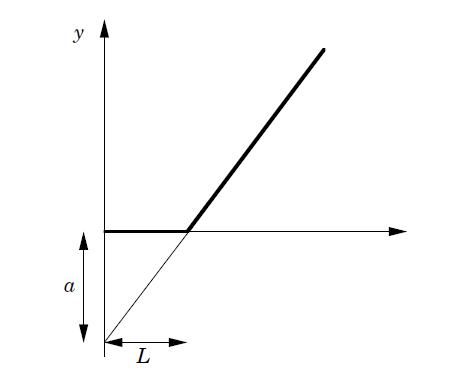
\includegraphics[scale=0.75]{img/ziegler-nichols_astrom_p135}
  \end{center}
  \fonte{\citeonline{Astrom1995}.} 
  \label{fig:ziegler-nichols_astrom_p135}
\end{figure}

Na tabela \ref{tab:Ziegler-Nichols} podemos ver as relações dos parâmetros $K_p$, $T_i$, $T_d$ e $T_p$ com os vistos na figura \ref{fig:ziegler-nichols_astrom_p135}.  

\begin{table}
  \caption{Parâmetros PID pelo Método de Ziegler-Nichols - Resposta ao Degrau}
  \label{tab:Ziegler-Nichols}
  \centering%
  \begin{minipage}{.42\textwidth}
    \begin{tabular*}{\textwidth}{lllll}
      \hline
      {Controlador} & {K} & {$T_i$} & {$T_d$}& {$T_p$}\\ \hline
      \hline
      P    &  1/a   &     &      & 4L  \\ 
      PI   &  0.9/a & 3L  &      & 5.7L  \\
      PID  &  1.2/a & 2L  & L/2  & 3.4L  \\ \hline
    \end{tabular*}
    \fonte{Adaptado de \citeonline{Astrom1995}}
  \end{minipage}
\end{table}

O outro método de se estimar os valores do controlador, é através de duas características da resposta em frequência: uma delas que é o ganho que deixa o sistema marginalmente estável ($K_u$), e a outra, é o período do sinal de referência que deixa o sistema marginalmente estável ($T_u$). Podemos ver na tabela \ref{tab:Ziegler-Nichols-freq} as relações entre $K_p$, $T_i$, $T_d$, $T_p$ e ($K_u$) e ($T_u$) . 

\begin{table}
  \caption{Parâmetros PID pelo Método de Ziegler-Nichols - Resposta em Frequência}
  \label{tab:Ziegler-Nichols-freq}
  \centering%
  \begin{minipage}{.52\textwidth}
    \begin{tabular*}{\textwidth}{lllll}
      \hline
      {Controlador} & {K} & {$T_i$} & {$T_d$}& {$T_p$}\\ \hline
      \hline
      P    &  0.5$K_u$   &           &             & $T_u$  \\ 
      PI   &  0.4$K_u$   & 0.8$T_u$  &             & 1.4$T_u$ \\
      PID  &  0.6$K_u$   & 0.5$T_u$  & 0.125$T_u$  & 0.85$T_u$  \\ \hline
    \end{tabular*}
    \fonte{Adaptado de \citeonline{Astrom1995}}
  \end{minipage}
\end{table}


%%%%%%%%%%%%%%%%%%%%%%%%%%%%%%%%%%%%%%%%%%%%%%%%%%%%%%%%%%%%%%%%%%%%%%

\subsection{Sintonia Automática de Controladores}

Como muitos sistemas sofrem variações temporais, distúrbios e o interesse do usuário em modificar constantemente a resposta da planta, cria-se a necessidade de automatizar o processo de sintonia, ao um simples comando do usuário.

Além da simplicidade do conceito de implementação, os controladores PID são muito utilizados pela possibilidade de auto sintonia e adaptatividade dos controladores, pois a partir do comportamento da resposta ao degrau podemos calcular os parâmetros do controlador e aplicarmos sem a intervenção humana\cite{Astrom1995}. Na figura \ref{fig:escolha_controle_astrom_p236}, podemos a partir do comportamento da planta, escolher a ou as técnicas mais adequadas que devemos implementar para controlar de forma satisfatória a planta.

\begin{figure}[!ht]
  \caption{Fluxograma para a escolha do Método de Sintonia.}
  \begin{center}
      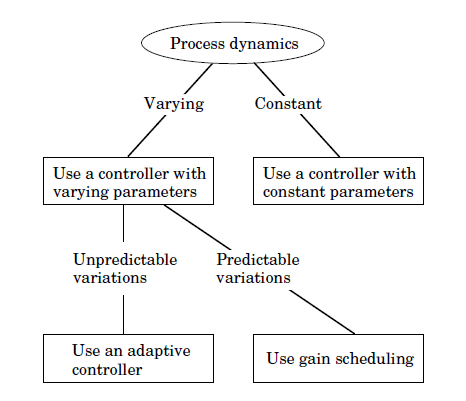
\includegraphics[scale=0.75]{img/escolha_controle_astrom_p236}
  \end{center}
  \fonte{Adaptado de \citeonline{Astrom1995}.} 
  \label{fig:escolha_controle_astrom_p236}
\end{figure}


%%%%%%%%%%%%%%%%%%%%%%%%%%%%%%%%%%%

\subsubsection{Método do Relé}

Características da resposta em frequência podem ser descobertas se somarmos ao sinal de referência, uma onda retangular ao mesmo tempo em que o controlador PID está desconectado. Esse é o princípio do método de sintonia usando relé, onde o relé desempenha o papel do chaveamento e cria um sinal retangular sobreposto ao sinal de referência \cite{Levine1996}. Na imagem \ref{fig:pid_autotuning_relay_astrom_p239} podemos ver o conceito básico do método do relé.
 
\begin{figure}[!ht]
  \caption{Modelo do Método de Auto Sintonia via Relé.}
  \begin{center}
      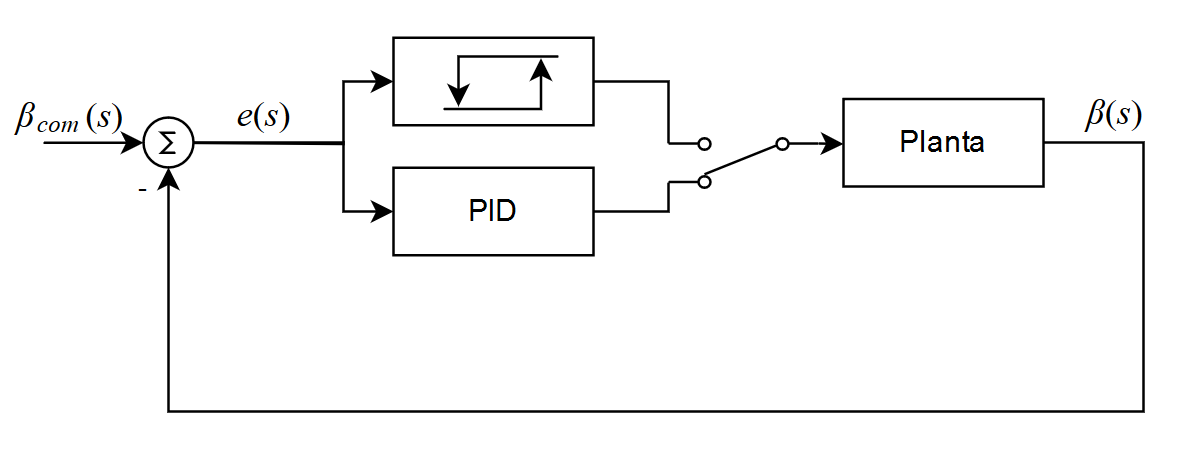
\includegraphics[scale=0.75]{img/pid_autotuning_relay_astrom_p239}
  \end{center}
  \fonte{Adaptado de \citeonline{Astrom1995}.} 
  \label{fig:pid_autotuning_relay_astrom_p239}
\end{figure}

O modelo matemático usado para descrever o comportamento de um relé, pode ser visto na equação da sequência:

\begin{equation}
  N(a)=\frac{4d}{\pi a}\left(\sqrt{1-\left(\frac{\varepsilon}{a}\right)^{2}}-i\frac{\varepsilon}{a}\right) 
\end{equation}

Onde \textit{d} é a amplitude de oscilação do relé (normalmente até 10\% do sinal de referência), \textit{$\varepsilon$} é a histerese do relé e \textit{a} é a amplitude do sinal de referencia \cite{Levine1996}. Isso pode ser visto na figura \ref{fig:relay_signals}.

\begin{figure}[!ht]
  \caption{Sinais do Relé e da Saída do Sistema  VOU COLOCAR OUTRA UMAGEM !!!!}
  \begin{center}
      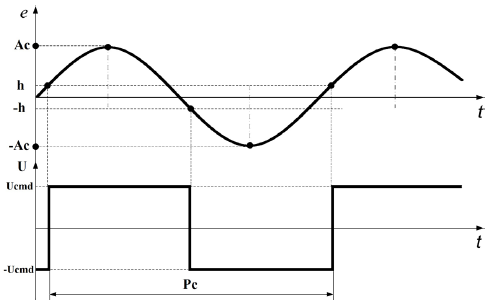
\includegraphics[scale=0.75]{img/relay_giap_p2}
  \end{center}
  \fonte{Adaptado de \citeonline{Giap2014}} 
  \label{fig:relay_signals}
\end{figure}

Com isso, podemos calcular os parâmetros intermediários para a sintonia do controlador da seguinte forma:

\begin{equation}
  K_u \approx \frac{4d}{\pi a} \\
  T_u = P_u
\end{equation}

Onde $P_u$ é o período de oscilação do sinal de interesse. Munido desses valores, podemos recorrer a tabela do método Ziegler-Nichols em resposta em frequência (Tabela \ref{tab:Ziegler-Nichols-freq}).


%%%%%%%%%%%%%%%%%%%%%%%%%%%%%%%%%%%

\subsection{Discretização e Processamento Digital de Sinais}

\begin{figure}[!ht]
  \caption{Resposta ao degrau com diferentes períodos de amostragem.}
  \begin{center}
      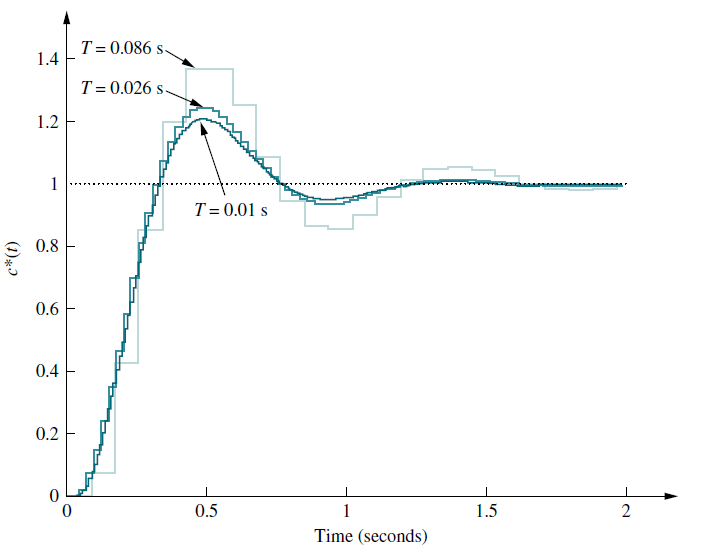
\includegraphics[scale=0.55]{img/nise_digitalinput_p761}
  \end{center}
  \fonte{Adaptado de \citeonline{Nise}.} 
  \label{fig:nise_digitalinput_p761}
\end{figure}


%%%%%%%%%%%%%%%%%%%%%%%%%%%%%%%%%%%%%%%%%%%%%%%%%%%%%%%%%%%%%%%%%%%%%%

\section{Linux Embarcados}

Linux embarcado  nada mais é do que uma versão do Kernel Linux que é desenvolvido para funcionar em um sistema embarcado, possuindo várias modificações para exigir menos recursos de processamento e memória \cite{Molloy2016}. Muitos dispositivos do nosso dia-a-dia possuem a implementação do Kernel do Linux em seu sistema, temos como exemplos os computadores pessoais, celulares com Android, televisores, entre outros. 

Na figura \ref{fig:componentes_linux_p13}, podemos ver a arquitetura de hardware de um sistema embarcado convencional. A arquitetura do processador é a RISC (Reduced Instruction Set Computer - Computador com um conjunto reduzido de instruções") de 32-bits. Possue dois tipos de memória, a SDRAM (Synchronous Dynamic Random-Access Memory - memória de acesso dinâmico randômico) que é volátil e a memória Flash que é usada para o armazenamento de informações persistentes. Possui RTC (Real Time Clock - relógio de tempo real), que nada mais é do que um relógio interno que funciona mesmo após desenergizar o embarcado, isso é possível devido a uma bateria ou um super-capacitor. Por fim, possue diversas interfaces de comunicação com outros dispositivos, entre elas: Porta serial, USB (Universal Serial Bus - Barramento serial universal), LAM (Local Area Network - Rede de área local) e Wi-Fi (rede sem fio) \citeonline{Prentice}.

\begin{figure}[!ht]
  \caption{Componentes básicos do Linux Embarcado}
  \begin{center}
      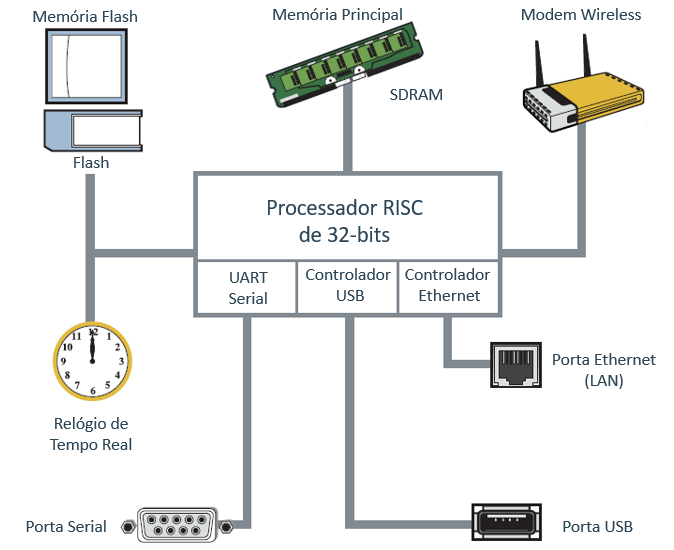
\includegraphics[scale=0.55]{img/componentes_linux_p13}
  \end{center}
  \fonte{Adaptado de \citeonline{Prentice}} 
  \label{fig:componentes_linux_p13}
\end{figure}

Quando nos referimos aos diferentes contextos de software em Linux, estamos falando do espaço de usuário e o espaço do Kernel. No espaço de usuário rodam as aplicações, já no espaço do Kernel, rodam as Threds e os acessos ao hardware. Os acessos entre regiões de memórias de um contexto pelo outro, são feitos através de chamadas de sistema do Kernel \cite{Prentice}. Essa estrutura pode ser vista na imagem \ref{fig:kernel_user_space}.

\begin{figure}[!ht]
  \caption{Estrutura Básica do Espaço de Usuário e de Kernel.}
  \begin{center}
      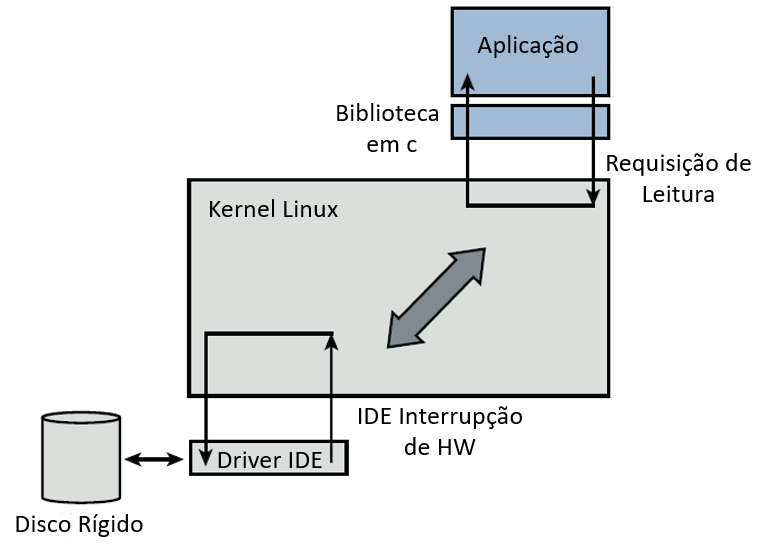
\includegraphics[scale=0.65]{img/kernel_user_space}
  \end{center}
  \fonte{Adaptado de \citeonline{Prentice}} 
  \label{fig:kernel_user_space}
\end{figure}


\begin{figure}[!ht]
  \caption{Linha do Tempo de execução de duas tarefas.}
  \begin{center}
      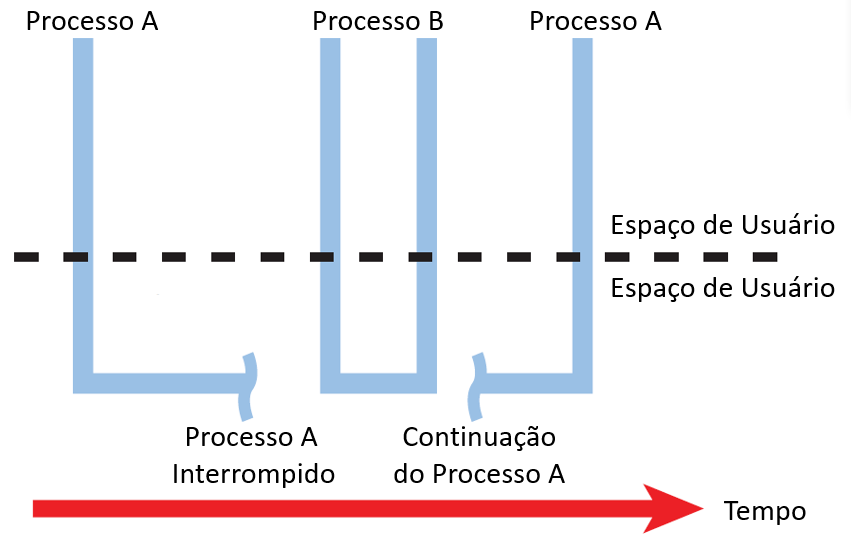
\includegraphics[scale=0.45]{img/escalonador_hallinan_p469}
  \end{center}
  \fonte{Adaptado de \citeonline{Prentice}} 
  \label{fig:escalonador_hallinan_p469}
\end{figure}
  
% \begin{figure}[!ht]
%   \caption{Representação do Modelo de Controlador PID com distúrbios}
%   \begin{center}
%       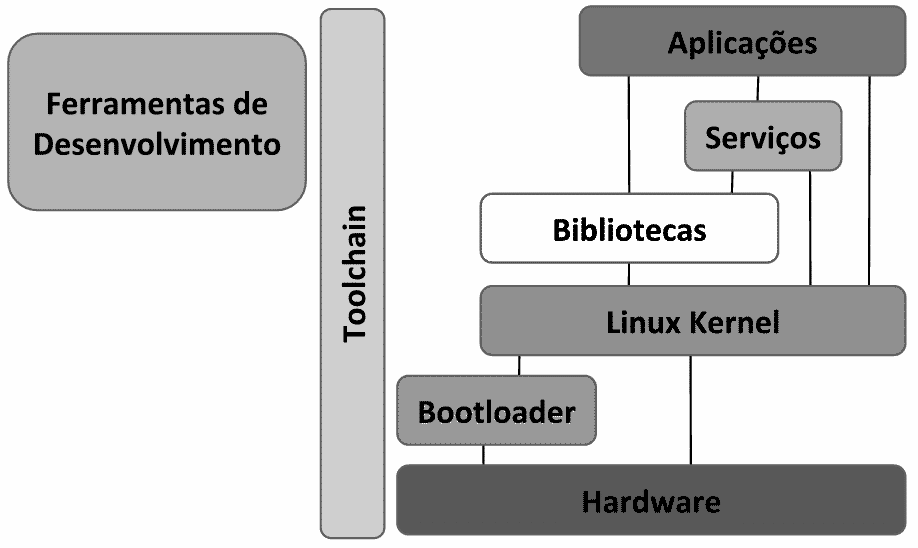
\includegraphics[scale=0.35]{img/sistema-linux-overview_embarcados}
%   \end{center}
%   \fonte{Adaptado de Embarcados....} 
%   \label{fig:sistema-linux-overview_embarcados}
% \end{figure}

%%%%%%%%%%%%%%%%%%%%%%%%%%%%%%%%%%%

\subsection{Linguagem de Programação Python}


%%%%%%%%%%%%%%%%%%%%%%%%%%%%%%%%%%%%%%%%%%%%%%%%%%%%%%%%%%%%%%%%%%%%%%

\section{Estado da Arte}


%%%%%%%%%%%%%%%%%%%%%%%%%%%%%%%%%%%

\subsection{Sistemas Inteligentes de Sintonia de Controladores}

\begin{figure}[!ht]
  \caption{Modelo de um Controlador com Auto-sintonia.}
  \begin{center}
      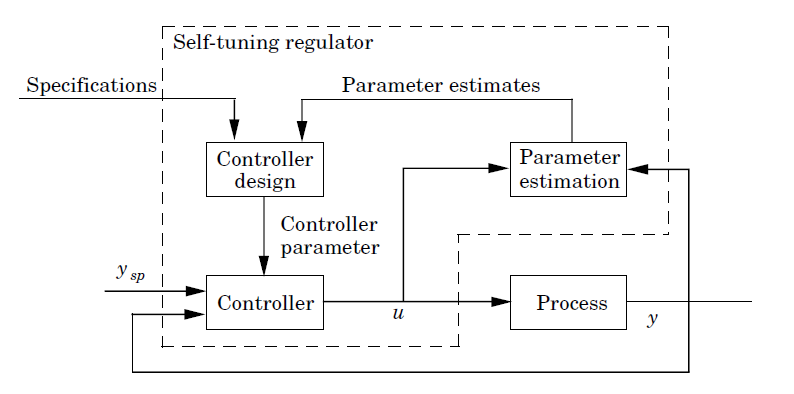
\includegraphics[scale=0.75]{img/pid_adaptative_astrom_p233}
  \end{center}
  \fonte{Adaptado de \citeonline{Astrom1995}.} 
  \label{fig:pid_adaptative_astrom_p233}
\end{figure}

%%%%%%%%%%%%%%%%%%%%%%%%%%%%%%%%%%%

\subsection{Controle Fuzzy} %Astrom p298


%%%%%%%%%%%%%%%%%%%%%%%%%%%%%%%%%%%

\subsection{Controle com Redes Neurais}  %control hand p1017

\begin{figure}[!ht]
  \caption{Modelo de um Simples Neurônio.}
  \begin{center}
      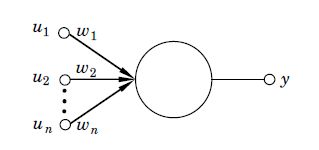
\includegraphics[scale=0.6]{img/neuron_astrom_p295}
  \end{center}
  \fonte{Adaptado de \citeonline{Astrom1995}.} 
  \label{fig:neuron_astrom_p295}
\end{figure}

\begin{figure}[!ht]
  \caption{Representação de uma Rede Neural.}
  \begin{center}
      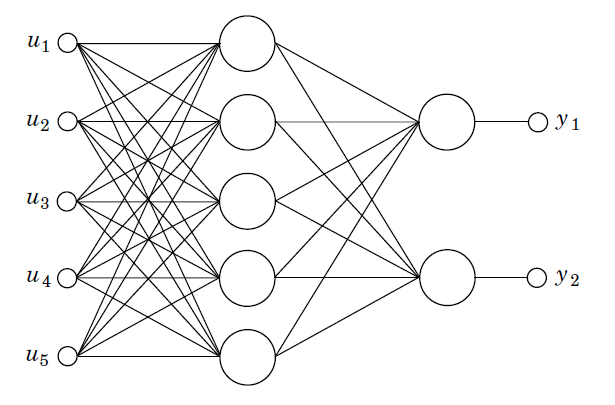
\includegraphics[scale=0.65]{img/feedforward_neural_astrom_p297}
  \end{center}
  \fonte{Adaptado de \citeonline{Astrom1995}.} 
  \label{fig:feedforward_neural_astrom_p297}
\end{figure}

\begin{figure}[!ht]
  \caption{Proposta de \citeonline{Chen2004} para um Controlador PID com Redes Neurais}
  \begin{center}
      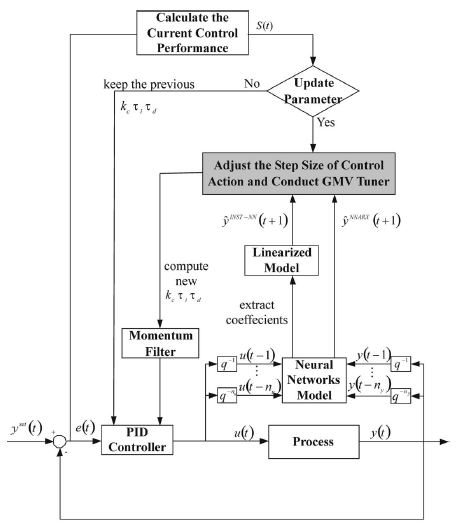
\includegraphics[scale=1]{img/pid_neural_Applying_p18}
  \end{center}
  \fonte{Adaptado de \citeonline{Chen2004}.} 
  \label{fig:pid_neural_Applying_p18}
\end{figure}
